\documentclass[11pt, a4paper]{article} % setsfont size and layout

%% required packages %%

\usepackage[margin=2.5cm]{geometry} % margins
\usepackage[english]{babel} % language (replace with german or ngerman for german texts)
\usepackage[utf8]{inputenc} % Umlaute
\usepackage{amsmath}		% math formulas
\usepackage{graphicx}		% graphics
\usepackage{fancyhdr}		% header and footer on every page
\usepackage{setspace}		% line space (e.g. \singlespacing, \onehalfspacing or \doublespacing)
\usepackage{xcolor}
\usepackage{subcaption}
\usepackage{pdflscape}
\usepackage{rotating}
%% Here the main part of the document begins %%

\begin{document}
	
%% Some more settings %%
	
\setlength{\parindent}{0pt} % first line in paragraph will not be indented
\onehalfspacing				% 1.5 line spacing
%\thispagestyle{empty}		% no header and page number on first page


%% Header on first page with course information etc. %%
\begin{tabular}{p{15.5cm}}
	{\large \textbf{Inrobin}} \\
	Gareth W. Peters  \\ 
	Dorota Toczydłowska\\
	Marta Campi\\
	\hline
	\\
\end{tabular}

\vspace*{0.3cm}				% vertical space between header on top of the page and main heading


\begin{center}
	{\LARGE \textbf{Experiment two:}}
	\vspace{2mm}	
\end{center} 

\section*{Unknown parameters - Frequency bands location}
Select one kernel family and take k elements from it corresponding to different hyperparameters sets (generated in Experiment 1). Take each set, aggregate the k elements together. Repeat this experiment for 1000 time-series. The procedure goes for each kernel considered in Experiment 1. That aggregation provides a synthetic observation set. Mathematically, it will be equivalent to simulate Gaussian Processes with mixture kernel. Once that 1000 time series are simulated, for each of them, we perform the EMD. For each IMF, take the IF and score the number of times it lies inside the partitions implied by the hyperparameters sets. Such frequency bands correspond to each kernel partition (histogram to do it). Do this for every replicate. Alternatively, we could do clustering on the frequency.\\ 

Stationary kernel considered:

\begin{itemize}

\item Square exponential. Hyperparameter: length scale $l$\\
\begin{equation*}
K(t,t')= \exp \left( - \frac{ \left( t - t' \right)^2 }{2 l^2} \right)
\end{equation*}

\item Periodic. Hyperparameters: length scale $l$, period $p$\\
\begin{equation*}
K(t,t')= \exp \left(  - \frac{2 \sin^2 \left( \pi (t - t')/p \right)}{l^2} \right)
\end{equation*}

\item Rational quadratic. Hyperparameters: length scale $l$, relative weighting of large-scale and small-scale variations $\alpha$. \\
\begin{equation*}
K(t,t') = \left(  1+ \frac{(t-t')^2}{2 \alpha l^2} \right)^{- \alpha} 
\end{equation*}

\item Locally periodic. Hyperparameters: square exponential and periodic kernels.\\
\begin{equation*}
K(t,t')= \exp \left(  - \frac{2 \sin^2 \left( \pi (t - t')/p \right)}{l^2} \right) \exp \left( - \frac{ \left( t - t' \right)^2 }{2 l^2} \right)
\end{equation*}

\end{itemize}



\newgeometry{top=1mm, bottom=1mm, left = 1mm, right = 1mm}
\begin{landscape}
\begin{figure*}
        \centering
        \begin{subfigure}[b]{0.475\hsize}\centering
            \centering
            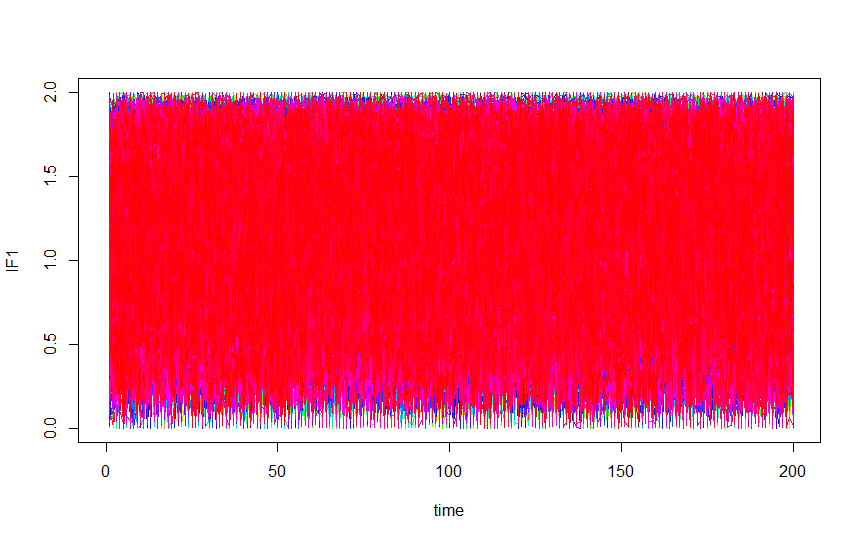
\includegraphics[width=0.8\textwidth]{IF1_Ex2.png}
            \caption[Periodic Kernel]%
            {{\small Instantaneous Frequency IMF1.}} 
        \end{subfigure}
        \quad
        \begin{subfigure}[b]{0.475\hsize}\centering
            \centering 
            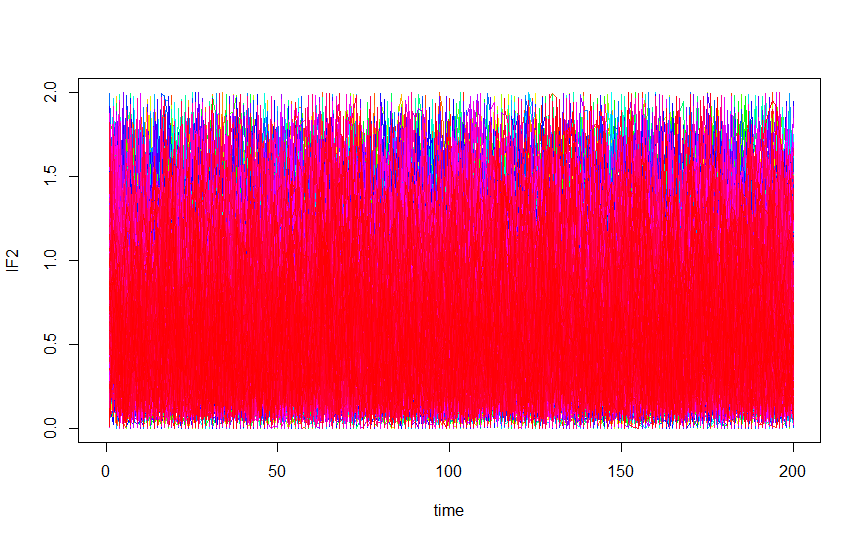
\includegraphics[width=0.8\textwidth]{IF2_Ex2.png}
            \caption[]%
            {{\small Instantaneous Frequency IMF2.}}    
        \end{subfigure}
        \\
        \begin{subfigure}[b]{0.475\hsize}\centering   
            \centering 
            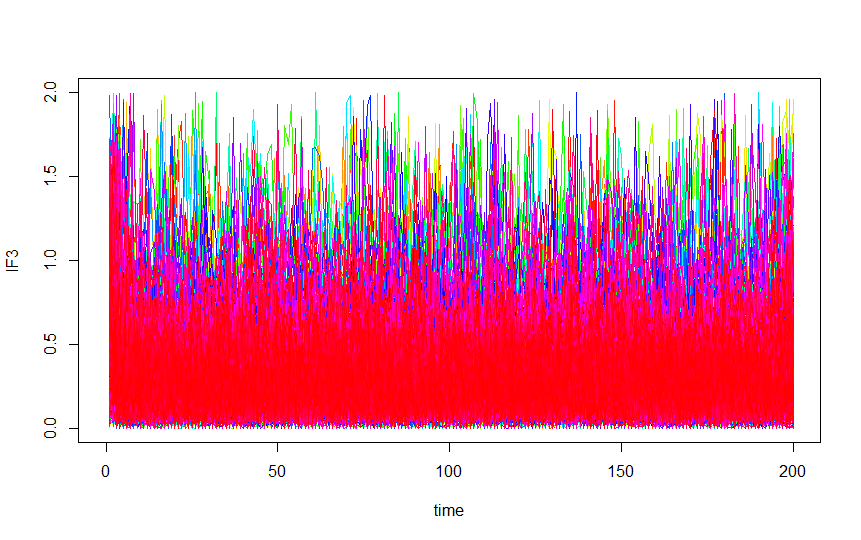
\includegraphics[width=0.8\textwidth]{IF3_Ex2.png}
            \caption[]%
            {{\small Instantaneous Frequency IMF3.}}
        \end{subfigure}
        \quad
        \begin{subfigure}[b]{0.475\hsize}\centering   
            \centering 
            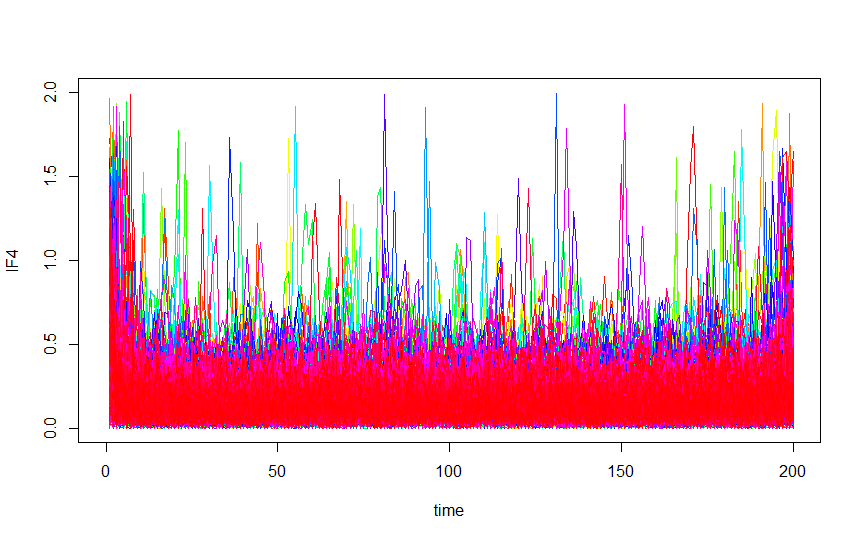
\includegraphics[width=0.8\textwidth]{IF4_Ex2.png}
            \caption[]%
            {{\small Instantaneous Frequency IMF4.}}
        \end{subfigure}
        \caption[  ]
        {\small Periodic Kernel. Instantaneous Frequencies of first,second, third and fourth IMFs extracted by the aggregated GP.} 
        \end{figure*}
\end{landscape}

\restoregeometry 

\end{document}